% Created by tikzDevice version 0.12 on 2018-09-28 04:16:46
% !TEX encoding = UTF-8 Unicode
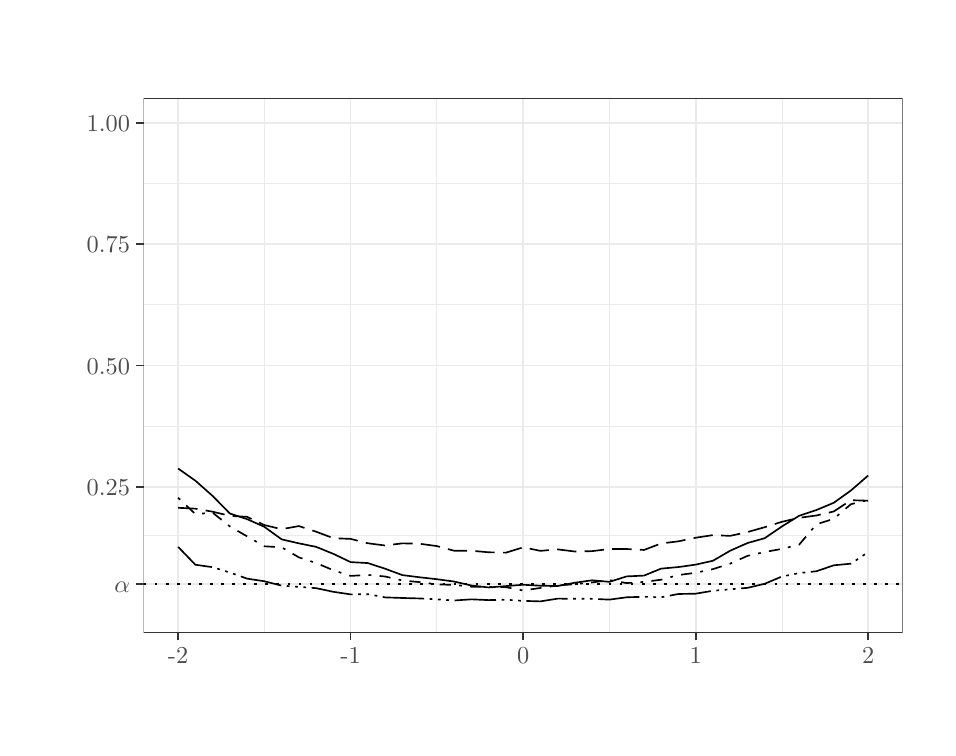
\begin{tikzpicture}[x=1pt,y=1pt]
\definecolor{fillColor}{RGB}{255,255,255}
\path[use as bounding box,fill=fillColor,fill opacity=0.00] (0,0) rectangle (325.21,252.94);
\begin{scope}
\path[clip] (  0.00,  0.00) rectangle (325.21,252.94);
\definecolor{drawColor}{RGB}{255,255,255}
\definecolor{fillColor}{RGB}{255,255,255}

\path[draw=drawColor,line width= 0.6pt,line join=round,line cap=round,fill=fillColor] (  0.00,  0.00) rectangle (325.21,252.94);
\end{scope}
\begin{scope}
\path[clip] ( 41.90, 34.26) rectangle (316.18,227.38);
\definecolor{fillColor}{RGB}{255,255,255}

\path[fill=fillColor] ( 41.90, 34.26) rectangle (316.18,227.38);
\definecolor{drawColor}{gray}{0.92}

\path[draw=drawColor,line width= 0.3pt,line join=round] ( 41.90, 69.37) --
	(316.18, 69.37);

\path[draw=drawColor,line width= 0.3pt,line join=round] ( 41.90,108.87) --
	(316.18,108.87);

\path[draw=drawColor,line width= 0.3pt,line join=round] ( 41.90,152.76) --
	(316.18,152.76);

\path[draw=drawColor,line width= 0.3pt,line join=round] ( 41.90,196.65) --
	(316.18,196.65);

\path[draw=drawColor,line width= 0.3pt,line join=round] ( 85.53, 34.26) --
	( 85.53,227.38);

\path[draw=drawColor,line width= 0.3pt,line join=round] (147.87, 34.26) --
	(147.87,227.38);

\path[draw=drawColor,line width= 0.3pt,line join=round] (210.21, 34.26) --
	(210.21,227.38);

\path[draw=drawColor,line width= 0.3pt,line join=round] (272.55, 34.26) --
	(272.55,227.38);

\path[draw=drawColor,line width= 0.6pt,line join=round] ( 41.90, 51.81) --
	(316.18, 51.81);

\path[draw=drawColor,line width= 0.6pt,line join=round] ( 41.90, 86.93) --
	(316.18, 86.93);

\path[draw=drawColor,line width= 0.6pt,line join=round] ( 41.90,130.82) --
	(316.18,130.82);

\path[draw=drawColor,line width= 0.6pt,line join=round] ( 41.90,174.71) --
	(316.18,174.71);

\path[draw=drawColor,line width= 0.6pt,line join=round] ( 41.90,218.60) --
	(316.18,218.60);

\path[draw=drawColor,line width= 0.6pt,line join=round] ( 54.37, 34.26) --
	( 54.37,227.38);

\path[draw=drawColor,line width= 0.6pt,line join=round] (116.70, 34.26) --
	(116.70,227.38);

\path[draw=drawColor,line width= 0.6pt,line join=round] (179.04, 34.26) --
	(179.04,227.38);

\path[draw=drawColor,line width= 0.6pt,line join=round] (241.38, 34.26) --
	(241.38,227.38);

\path[draw=drawColor,line width= 0.6pt,line join=round] (303.71, 34.26) --
	(303.71,227.38);
\definecolor{drawColor}{RGB}{0,0,0}

\path[draw=drawColor,line width= 0.6pt,dash pattern=on 1pt off 3pt on 4pt off 3pt ,line join=round] ( 54.37, 83.06) --
	( 60.60, 77.17) --
	( 66.83, 77.69) --
	( 73.07, 72.71) --
	( 79.30, 69.12) --
	( 85.53, 65.54) --
	( 91.77, 65.16) --
	( 98.00, 61.54) --
	(104.24, 59.50) --
	(110.47, 56.87) --
	(116.70, 54.83) --
	(122.94, 55.19) --
	(129.17, 54.62) --
	(135.40, 53.18) --
	(141.64, 52.59) --
	(147.87, 51.78) --
	(154.10, 51.57) --
	(160.34, 50.94) --
	(166.57, 50.90) --
	(172.81, 50.76) --
	(179.04, 49.57) --
	(185.27, 50.48) --
	(191.51, 51.39) --
	(197.74, 51.85) --
	(203.97, 52.48) --
	(210.21, 53.32) --
	(216.44, 52.24) --
	(222.68, 52.66) --
	(228.91, 53.46) --
	(235.14, 55.15) --
	(241.38, 55.96) --
	(247.61, 57.29) --
	(253.84, 59.26) --
	(260.08, 62.07) --
	(266.31, 63.47) --
	(272.55, 64.60) --
	(278.78, 66.14) --
	(285.01, 73.48) --
	(291.25, 75.45) --
	(297.48, 80.75) --
	(303.71, 82.26);

\path[draw=drawColor,line width= 0.6pt,dash pattern=on 15pt off 2pt on 1pt off 2pt on 1pt off 2pt on 1pt off 2pt ,line join=round] ( 54.37, 65.33) --
	( 60.60, 58.87) --
	( 66.83, 57.99) --
	( 73.07, 56.06) --
	( 79.30, 53.85) --
	( 85.53, 52.90) --
	( 91.77, 51.32) --
	( 98.00, 50.87) --
	(104.24, 50.41) --
	(110.47, 49.08) --
	(116.70, 48.16) --
	(122.94, 48.23) --
	(129.17, 47.07) --
	(135.40, 46.86) --
	(141.64, 46.69) --
	(147.87, 46.37) --
	(154.10, 45.95) --
	(160.34, 46.37) --
	(166.57, 46.09) --
	(172.81, 46.23) --
	(179.04, 45.81) --
	(185.27, 45.63) --
	(191.51, 46.62) --
	(197.74, 46.58) --
	(203.97, 46.55) --
	(210.21, 46.27) --
	(216.44, 47.11) --
	(222.68, 47.29) --
	(228.91, 47.11) --
	(235.14, 48.30) --
	(241.38, 48.41) --
	(247.61, 49.46) --
	(253.84, 49.99) --
	(260.08, 50.52) --
	(266.31, 51.99) --
	(272.55, 54.62) --
	(278.78, 55.85) --
	(285.01, 56.52) --
	(291.25, 58.66) --
	(297.48, 59.26) --
	(303.71, 63.44);

\path[draw=drawColor,line width= 0.6pt,dash pattern=on 7pt off 3pt ,line join=round] ( 54.37, 79.45) --
	( 60.60, 79.13) --
	( 66.83, 78.04) --
	( 73.07, 76.53) --
	( 79.30, 76.18) --
	( 85.53, 73.20) --
	( 91.77, 71.72) --
	( 98.00, 72.85) --
	(104.24, 70.81) --
	(110.47, 68.46) --
	(116.70, 68.21) --
	(122.94, 66.63) --
	(129.17, 65.82) --
	(135.40, 66.60) --
	(141.64, 66.46) --
	(147.87, 65.61) --
	(154.10, 63.93) --
	(160.34, 63.93) --
	(166.57, 63.37) --
	(172.81, 63.23) --
	(179.04, 65.16) --
	(185.27, 63.89) --
	(191.51, 64.42) --
	(197.74, 63.65) --
	(203.97, 63.79) --
	(210.21, 64.56) --
	(216.44, 64.56) --
	(222.68, 64.21) --
	(228.91, 66.56) --
	(235.14, 67.33) --
	(241.38, 68.63) --
	(247.61, 69.58) --
	(253.84, 69.30) --
	(260.08, 70.67) --
	(266.31, 72.43) --
	(272.55, 74.39) --
	(278.78, 75.83) --
	(285.01, 76.67) --
	(291.25, 78.11) --
	(297.48, 82.19) --
	(303.71, 82.01);

\path[draw=drawColor,line width= 0.6pt,line join=round] ( 54.37, 93.63) --
	( 60.60, 89.24) --
	( 66.83, 83.73) --
	( 73.07, 77.38) --
	( 79.30, 75.34) --
	( 85.53, 72.57) --
	( 91.77, 68.04) --
	( 98.00, 66.60) --
	(104.24, 65.33) --
	(110.47, 62.80) --
	(116.70, 59.82) --
	(122.94, 59.47) --
	(129.17, 57.43) --
	(135.40, 55.12) --
	(141.64, 54.34) --
	(147.87, 53.64) --
	(154.10, 52.80) --
	(160.34, 51.36) --
	(166.57, 50.66) --
	(172.81, 51.15) --
	(179.04, 51.64) --
	(185.27, 51.29) --
	(191.51, 51.18) --
	(197.74, 52.38) --
	(203.97, 53.25) --
	(210.21, 52.69) --
	(216.44, 54.66) --
	(222.68, 54.94) --
	(228.91, 57.47) --
	(235.14, 58.03) --
	(241.38, 58.91) --
	(247.61, 60.31) --
	(253.84, 63.93) --
	(260.08, 66.70) --
	(266.31, 68.46) --
	(272.55, 72.71) --
	(278.78, 76.57) --
	(285.01, 78.64) --
	(291.25, 81.24) --
	(297.48, 85.70) --
	(303.71, 91.11);

\path[draw=drawColor,line width= 0.6pt,dash pattern=on 1pt off 3pt ,line join=round] ( 41.90, 51.81) -- (316.18, 51.81);
\definecolor{drawColor}{gray}{0.20}

\path[draw=drawColor,line width= 0.6pt,line join=round,line cap=round] ( 41.90, 34.26) rectangle (316.18,227.38);
\end{scope}
\begin{scope}
\path[clip] (  0.00,  0.00) rectangle (325.21,252.94);
\definecolor{drawColor}{gray}{0.30}

\node[text=drawColor,anchor=base east,inner sep=0pt, outer sep=0pt, scale=  0.88] at ( 36.95, 48.78) {$\alpha$};

\node[text=drawColor,anchor=base east,inner sep=0pt, outer sep=0pt, scale=  0.88] at ( 36.95, 83.90) {$0.25$};

\node[text=drawColor,anchor=base east,inner sep=0pt, outer sep=0pt, scale=  0.88] at ( 36.95,127.79) {$0.50$};

\node[text=drawColor,anchor=base east,inner sep=0pt, outer sep=0pt, scale=  0.88] at ( 36.95,171.68) {$0.75$};

\node[text=drawColor,anchor=base east,inner sep=0pt, outer sep=0pt, scale=  0.88] at ( 36.95,215.57) {$1.00$};
\end{scope}
\begin{scope}
\path[clip] (  0.00,  0.00) rectangle (325.21,252.94);
\definecolor{drawColor}{gray}{0.20}

\path[draw=drawColor,line width= 0.6pt,line join=round] ( 39.15, 51.81) --
	( 41.90, 51.81);

\path[draw=drawColor,line width= 0.6pt,line join=round] ( 39.15, 86.93) --
	( 41.90, 86.93);

\path[draw=drawColor,line width= 0.6pt,line join=round] ( 39.15,130.82) --
	( 41.90,130.82);

\path[draw=drawColor,line width= 0.6pt,line join=round] ( 39.15,174.71) --
	( 41.90,174.71);

\path[draw=drawColor,line width= 0.6pt,line join=round] ( 39.15,218.60) --
	( 41.90,218.60);
\end{scope}
\begin{scope}
\path[clip] (  0.00,  0.00) rectangle (325.21,252.94);
\definecolor{drawColor}{gray}{0.20}

\path[draw=drawColor,line width= 0.6pt,line join=round] ( 54.37, 31.51) --
	( 54.37, 34.26);

\path[draw=drawColor,line width= 0.6pt,line join=round] (116.70, 31.51) --
	(116.70, 34.26);

\path[draw=drawColor,line width= 0.6pt,line join=round] (179.04, 31.51) --
	(179.04, 34.26);

\path[draw=drawColor,line width= 0.6pt,line join=round] (241.38, 31.51) --
	(241.38, 34.26);

\path[draw=drawColor,line width= 0.6pt,line join=round] (303.71, 31.51) --
	(303.71, 34.26);
\end{scope}
\begin{scope}
\path[clip] (  0.00,  0.00) rectangle (325.21,252.94);
\definecolor{drawColor}{gray}{0.30}

\node[text=drawColor,anchor=base,inner sep=0pt, outer sep=0pt, scale=  0.88] at ( 54.37, 23.25) {-2};

\node[text=drawColor,anchor=base,inner sep=0pt, outer sep=0pt, scale=  0.88] at (116.70, 23.25) {-1};

\node[text=drawColor,anchor=base,inner sep=0pt, outer sep=0pt, scale=  0.88] at (179.04, 23.25) {0};

\node[text=drawColor,anchor=base,inner sep=0pt, outer sep=0pt, scale=  0.88] at (241.38, 23.25) {1};

\node[text=drawColor,anchor=base,inner sep=0pt, outer sep=0pt, scale=  0.88] at (303.71, 23.25) {2};
\end{scope}
\end{tikzpicture}
